%\immediate\write18{bibtex \jobname}
\documentclass[nospthms, a4paper, final]{svjour3}
\setlength{\textwidth}{\dimexpr\pdfpagewidth-2in}
\setlength{\textheight}{\dimexpr\pdfpageheight-2in}
\usepackage{mathptmx}
\usepackage{amsmath, amsthm, amssymb}
\usepackage{tikz-cd}
\usepackage[numbers,sort,compress]{natbib}
\usepackage{graphicx}
\usepackage{csquotes}
\usepackage[bookmarks=true,
bookmarksnumbered=true, breaklinks=true,
pdfstartview=FitH, hyperfigures=true,
plainpages=false, naturalnames=true,
colorlinks=true, pagebackref=true,
pdfpagelabels]{hyperref}
\hypersetup{
	linktocpage,
	colorlinks,
	citecolor=blue,
	linkcolor=blue,
	urlcolor=blue}
\usepackage[capitalize, noabbrev]{cleveref}
\usepackage{todo}

% theorems
\theoremstyle{plain}
\newtheorem{thm}{Theorem}[section]
\Crefname{thm}{Theorem}{Theorems}
\newtheorem{cor}[thm]{Corollary}
\newtheorem{lem}[thm]{Lemma}
\newtheorem{prop}[thm]{Proposition}
\Crefname{prop}{Proposition}{Propositions}
\newtheorem{claim}[thm]{Claim}
\newtheorem{conj}[thm]{Conjecture}
\Crefname{conj}{Conjecture}{Conjectures}
\theoremstyle{definition}
\newtheorem{defi}[thm]{Definition}
\newtheorem{ex}[thm]{Example}
\newtheorem{rem}[thm]{Remark}

% commands
\newcommand{\N}{\mathbb{N}}
\newcommand{\Z}{\mathbb{Z}}
\newcommand{\F}{\mathbb{F}}
\newcommand{\R}{\mathbb{R}}
\newcommand{\HS}{\mathrm{HS}}
\newcommand{\HT}{\mathrm{HT}}
\newcommand{\HLC}{\mathrm{LHS}}
\newcommand{\piT}{\pi\mathrm{T}}
\newcommand{\LC}{\mathrm{LC}}
\newcommand{\NH}{\mathrm{NH}}
\newcommand{\piLC}{\pi\mathrm{LC}}
\newcommand{\HE}{\mathbb{H}^d}
\renewcommand{\H}{H}
\DeclareMathOperator{\interior}{int}
\DeclareMathOperator{\im}{im}
\DeclareMathOperator{\coker}{coker}
\DeclareMathOperator{\rad}{rad}
\newcommand\CH{\check{H}}
\newcommand{\Mod}[1]{#1-\mathbf{Mod}}
\newcommand{\PFD}{\mathrm{PFD}}
\newcommand{\PFG}{\mathrm{PFG}}
\DeclareMathOperator{\Nrv}{Nrv}
\DeclareMathOperator{\Cov}{Cov}
\DeclareMathOperator{\Vietoris}{Vtr}
\DeclareMathOperator{\Balls}{Balls}
\DeclareMathOperator*{\colim}{colim}
\DeclareMathOperator{\crit}{crit}
\newcommand\MCH{M\check{H}}
\newcommand\VH{VH}
\newcommand\MVH{MVH}
\newcommand{\obs}{\dashrightarrow}
\newcommand{\multiplicityDomain}{\mathcal{E}}
\newcommand{\Top}{\mathsf{Top}}
\newcommand{\Vect}{\mathsf{Vect}}
\renewcommand{\th}{^{\mathrm{th}}}
\newcommand{\anibal}[1]{\textcolor{blue}{\underline{Anibal}: #1}}

\begin{document}

\title{Persistence in functional topology and a correction to a theorem of Morse}

\author{Ulrich Bauer \and Anibal M.~Medina-Mardones \and Maximilian Schmahl}

\institute{
    Ulrich Bauer \at Technical University of Munich \\ \email{mail@ulrich-bauer.org} \and
	Anibal M.~Medina-Mardones \at Max Planck Institute for Mathematics in Bonn \at Department of Mathematics, University of Notre Dame \\ \email{ammedmar@mpim-bonn.mpg.de} 
	\and
	Maximilian Schmahl \at Heidelberg University \\ \email{mschmahl@mathi.uni-heidelberg}
}

\authorrunning{U.~Bauer, A.~Medina-Mardones, M.~Schmahl}

\maketitle

\begin{abstract}
	During the 1930s, Marston Morse developed a vast generalization of what is commonly known as Morse theory relating the critical points of a semi-continuous functional with the topology of its sublevel sets.
	Morse and Tompkins applied this body of work, referred to as functional topology, to prove the Unstable Minimal Surface Theorem in the setting defined by Douglas' solution to Plateau's Problem.
	Several concepts introduced by Morse in this context can be seen as early precursors to the theory of persistent homology, which by now has established itself as a popular tool in applied and theoretical mathematics with applications to a wide range of topics, including neuroscience, genomics, and symplectic geometry.
	In this article, we provide a modern redevelopment of the homological aspects of Morse's functional topology from the perspective of persistence theory.
	We adjust several key definitions and prove stronger statements in order to allow for future applications of persistence techniques in functional analysis, as well as to correct a mistake in the proof by Morse and Tompkins of the Unstable Minimal Surface Theorem.
\end{abstract}

\tableofcontents
%!TEX root = ../func_top.tex

\section{Introduction}

The interplay between the critical set of a function and the topology of its domain is a cornerstone of modern mathematics.
Nowadays, when thinking about the pioneering work of Marston Morse, our first thought probably involves a differentiable function on a closed smooth manifold, but more general settings should also be considered.
Morse theory in the smooth context was masterfully presented in Milnor's famous book on the subject \cite{Milnor.1963}, where he also gave a new proof of Bott's periodicity by applying Morse theory to the energy functional of paths in a Riemannian manifold, which notably goes beyond the compact setting.
Another important example of the use of Morse's insights in an infinite-dimensional context is Floer's work on the Arnold conjecture and its many ramifications in symplectic topology, as surveyed for example in \cite{Salamon.1999}.
Morse himself worked in a very general setting, publishing in the 1930s a pair of papers \cite{Morse.1937, Morse.1940} and a monograph \cite{Morse.1938} in which he established the key results of Morse theory in the broad context defined by semi-continuous functionals on metric spaces.
He called the theory set forth in this body of work \emph{functional topology} and used it to study questions about minimal surfaces motivated by Douglas' solution to Plateau’s Problem \cite{Douglas.1931}.
In particular, Morse and Tompkins \cite{Morse.1939} used these techniques to prove a general \emph{Mountain Pass Theorem} --~an existence result for saddle points~-- applying to functions that are not necessarily continuous (\cref{thm:mountain_pass}).
From this, they deduce their \emph{Unstable Minimal Surface Theorem}, showing the existence of critical points of the Douglas functional that are not local minima (\cref{thm:unstable_minimial_surface}).
In the intervening years, this result has been reproven and generalized in several directions using various techniques, and the problem class is still an active area of research \cite{Struwe.1984,Jost.1990,Jost.1991,Montezuma.2020,Marques.2021}.

Morse's work on functional topology did not have a long lasting impact on minimal surface theory or the calculus of variations in general; possibly in part because, as expressed by Struwe:
\begin{displaycquote}[p.~82]{Struwe.1988}
	The technical complexity and the use of a sophisticated topological machinery [...] tend to make Morse--Tompkins' original paper unreadable and inaccessible for the non-specialist.
\end{displaycquote}
A similar assessment was given by Bott, who writes in \cite[p.~934]{Bott.1980} that the papers \cite{Morse.1937, Morse.1940} ``are not easy reading'' and constitute a ``tour de force'' by Morse.

The intricacies of Morse's development notwithstanding, many of his ideas have subsequently resurfaced and flourished in other domains.
In particular, in applied topology and symplectic geometry, several key insights of Morse have been independently rediscovered as part of the development of \emph{persistent homology}, a technique that provides robust and efficiently computable invariants of filtered spaces using the functorial properties of homology.
Its success in these fields has motivated a refined abstract theory of persistence that lies in the intersection of geometry, topology, and representation theory.

The homology of a filtered space is an example of what is referred to as a \emph{persistence module}, a functor to vector spaces from the real numbers considered as a poset category.
In many important cases, a persistence module $M$ admits an essentially unique decomposition into indecomposable direct summands, and the structure of this decomposition yields a complete invariant of $M$ known as its \emph{persistence diagram}.
The set of all persistence diagrams can be organized into a metric space.
This often allows to recast geometric questions about general filtered spaces in a combinatorial metric model, since the passage via the homology construction to this metric space is Lipschitz, a statement commonly known as the \emph{stability} of persistence diagrams.

The most remarkable connections between functional topology and persistence theory come from Morse's paper \cite{Morse.1940}, where he developed the theory of \emph{caps} and their \emph{spans}.
They capture much of the same information as the modern notion of persistence diagram, including concepts such as the persistence or birth and death of a homology class, although Morse's results still fall short of yielding global decompositions of persistence modules.
Morse used his theory of caps to study functionals on a metric space by analyzing the evolution of the topology of their sublevel sets.
A key tool to this end is a version of his eponymous inequalities for cap numbers, which expands their usual version in the compact and smooth setting.
In this work, using persistence diagrams, we generalize the definition of these cap numbers to persistence modules and prove the existence of Morse inequalities for a large class of them (\cref{t:inequalities}).
Our approach makes these inequalities accessible in new contexts beyond those originally covered by functional topology.

Given the importance of persistence diagrams, in particular for stating and proving Morse inequalities, our focus will then be on the study of topological properties ensuring their existence for a broad class of filtered spaces and homology constructions.
For general persistence modules, a well studied condition for the existence of persistence diagrams is \emph{q-tameness} \cite{Chazal.2016a,Chazal.2016b}, which simply states that all linear maps between different real values in the persistence module have finite rank.
This condition is satisfied by a large class of important constructions; for example, the Vietoris--Rips or \v Cech persistent homology of a totally bounded metric space is q-tame \cite{Chazal.2014}.
The motivating question can then be reformulated as asking for topological conditions on a filtered space that ensure its persistent homology to be q-tame.
We now present the answers provided in the present work.

The persistence module associated to a filtration depends on the homology construction used, which, even when agreeing on cellular spaces, need not coincide for general topological spaces.
We restrict attention to homotopy invariant functors to the category of graded vector spaces satisfying the Mayer--Vietoris property for either open or closed sets, the primary examples being singular homology and \v{C}ech homology, respectively.

The sublevel set filtration $f_{\leq t} = f^{-1}(-\infty, t]$ of a real valued function $f$ is called \emph{locally homologically small} or \emph{$\HLC$} for a given homology theory if for any $x \in X$, any neighborhood $V$ of $x$, and any pair of indices $s,t$ with $f(x) < s < t$, there is a neighborhood $U$ of $x$ with $U \subseteq V$ such that the inclusion $f_{\leq s} \cap U \hookrightarrow f_{\leq t} \cap V$ is \emph{homologically small}; that is to say, the induced map in homology has finite rank in every degree.
We say that a sublevel set filtration is \emph{compact} if all sublevel sets are compact Hausdorff spaces.
We can now state our main result (\cref{t:local connectedness implies q-tameness}):

\begin{thm*}
	If the sublevel set filtration of a function $f \colon X \to \R$ is compact and	$\HLC$, then its persistent homology is q-tame.
\end{thm*}

\noindent We also introduce a weaker local-connectivity condition that can be used instead of $\HLC$ in the statement above if the filtration is defined by a continuous functional (\cref{c:q-tameness for continuous functions}).

To illustrate the applicability of our results we return to the original setting of the Douglas functional that motivated the development of functional topology.
This functional satisfies the hypotheses of \cref{t:local connectedness implies q-tameness}, so its associated persistent \v{C}ech homology is indeed q-tame and admits a persistence diagram.
From this, one can easily deduce the existence of an unstable minimal surface.
As it turns out, the local connectivity conditions proposed by Morse \cite{Morse.1938,Morse.1939,Morse.1940} are not sufficient for this purpose, which we illustrate by a counterexample (\cref{c:counterexample}).


\subsection*{Summary}

The primary contribution of this work consists in a modern development of the homological aspects of Morse's functional topology from the perspective of persistence theory.
We adjust several key definitions and prove stronger statements -- including a generalized version of the Morse inequalities -- in order to allow for novel uses of persistence techniques in the calculus of variations.
We provide sufficient conditions for a lower semicontinuous function to have q-tame persistent sublevel set homology, and hence to admit a persistence diagram.
As an application of these results, we correct an inaccuracy in a result by Morse, which was employed in the proof of the Unstable Minimal Surface Theorem given by Morse and Tompkins.


\subsection*{Outline}

In \cref{s:persistence} we recall the foundations of persistence theory, considering the persistent homology of a sublevel set filtration as the key example.
We present a persistence-theoretic point of view on Morse inequalities in \cref{s:inequalities}.
It generalizes both their versions in the smooth and compact setting as well as the one used in functional topology.
The main result of the present work is presented in \cref{s:connectivity}, where we define two natural notions of local-connectivity for a sublevel set filtration and show under what circumstances they imply q-tameness of its associated persistence module.
We close in \cref{s:surfaces} with a historical overview of Morse--Tompkins' application of functional topology to minimal surface theory, and we explore its relation to our results.
\cref{s:vietoris} contains a brief discussion on the definitions of Vietoris and \v{C}ech homology and their equivalence for compact metric spaces.

%!TEX root = ../func_top.tex

\section{Filtered spaces and persistence theory} \label{s:persistence}

In this section we present an overview of the theory of persistence through filtrations by sublevel sets of real-valued functions on general topological spaces.
For a detailed exposition we refer to \cite{Chazal.2016a, Oudot.2015, Polterovich.2020} and for applications of this theory in symplectic geometry to
\cite{Polterovich.2016, Usher.2016, LeRoux.2018, Shelukhin.2019}.

The ``pipeline'' of topological persistence traverses through geometry, algebra and discrete mathematics as follows:
Given a space $X$ filtered by the sublevel sets of a function $f$, the application of some homology theory in degree $n$ with coefficients in a field, or, more generally, a functor from topological spaces to vector spaces, produces a \emph{persistence module}, an algebraic object equipped with a structure theory leading in favorable cases to a powerful invariant called \emph{persistence diagram}.

These invariants are key to applications.
For example, in the next section we will see how they lead to a generalization of the classical Morse inequalities.
Much of their usefulness results from a remarkable fact known as \emph{stability}, stating that the map from functions on $X$ with the supremum norm to the set of all persistence diagrams is 1-Lipschitz with respect to a certain natural metric called \emph{bottleneck distance} \cite{Cohen-Steiner.2007}.

In more detail, consider a space $X$ and a function $f \colon X \to \R$.
Unless stated otherwise, the functions we consider need not be continuous.
We pass to filtered spaces by considering the \emph{sublevel set filtration $f_{\leq \bullet}$ of $X$ induced by $f$}, which is defined by
\begin{equation*}
f_{\leq t} = f^{-1}(-\infty, t].
\end{equation*}

For the next step in the persistence pipeline, one needs a coherent assignment of a vector space to any topological space, or, more precisely, a functor from the category $\Top$ of topological spaces to the category $\Vect$ of vector spaces over a fixed field $\F$.
The typical choices are given by \emph{homology theories}, which for now are only assumed to be $\Z$-graded families $\H = (\H_d)_{d \in \Z}$ of \emph{homotopy invariant functors}, meaning that they assign the same morphism to homotopic maps.
Of particular importance to us are \v{C}ech homology \cite[Section IX--X]{Eilenberg.1952} with coefficients in $\F$, and homology theories in the sense of Eilenberg--Steenrod \cite[Section I]{Eilenberg.1952}, such as singular homology, again with coefficients in $\F$ \cite{Eilenberg.1944}.

By definition, applying to a filtered space $\{X_t\}_{t \in \R}$ a functor from $\Top$ to $\Vect$ yields, for every $t \in \R$ a vector space~$M_t$ and for any pair~$s, t \in \R$ with~$s \leq t$, a linear map~$M_{s,t} \colon M_s \to M_t$ such that $M_{t,t}$ is the identity and the composition $M_{s,t} \circ M_{r,s}$ is equal to $M_{r,t}$ for any triple $r \leq s \leq t$.
In other words, we obtain a functor $M$ from the real numbers, considered as a poset category, to the category of vector spaces.
Such functors are called \emph{persistence modules}.
A morphism of persistence modules $\varphi \colon M \to N$ is a natural transformation, i.e., an assignment of a linear map $\varphi_t \colon M_t \to N_t$ for every $t \in \R$ making the diagram
\begin{equation*}
\begin{tikzcd}
M_{s} \arrow[r, "M_{s,t}"] \arrow[d] & M_{t} \arrow[d] \\
N_{s} \arrow[r, "N_{s,t}"] & N_{t}
\end{tikzcd}
\end{equation*}
commute for every pair $s \leq t$.

Since most examples of interest arise from applying a homology theory to a filtered space, we also consider \emph{graded persistence modules}, which are collections of persistence modules indexed by the integers.
To lighten the presentation of the theory of persistence, in what follows we will solely focus on persistence modules, omitting straightforward generalizations to their graded counterparts.

Functorial constructions defined on the category of vector spaces over the field~$\F$ can be transferred to the category of persistence modules by applying them pointwise.
For example, the kernel and cokernel of a morphism as well as the direct sum of persistence modules are well-defined.
Persistence modules that are \emph{indecomposable}, i.e., those that have only trivial direct sum decompositions, play an important role in persistence theory.
A rich family of indecomposable persistence modules is given by \emph{interval modules}, which for intervals $I \subseteq \R$ are defined by
\begin{equation*}
C(I)_t =
\begin{cases}
\F & \text{if } t \in I, \\
0 & \text{otherwise},
\end{cases}
\qquad \qquad
C(I)_{s, t} =
\begin{cases}
\operatorname{id}_{\F} & \text{if } s, t \in I, \\
0 & \text{otherwise}.
\end{cases}
\end{equation*}
These indecomposable interval modules can be used as building blocks for \emph{barcode modules}, which are direct sums of interval modules.
Given a barcode module $\bigoplus_{\lambda \in \Lambda} C(I_{\lambda})$, the associated multiset of intervals $\{I_{\lambda}\}_{\lambda \in \Lambda}$ is known as its \emph{barcode}.
By a version of the Krull--Remak--Schmidt--Azumaya Theorem \cite{Azumaya.1950} (see also \cite[Theorem 2.7]{Chazal.2016a} for a specialization to barcode modules), two isomorphic barcode modules have the same barcodes up to a choice of the index set $\Lambda$.
Thus, if a persistence module $M$ is provided with an isomorphism to a barcode module, referred to as a \emph{barcode decomposition}, the associated barcode is a complete isomorphism invariant of $M$.
Hence, understanding which persistence modules admit barcode decompositions is key.

The most commonly used existence result for barcode decompositions is due to Crawley-Boevey \cite{Crawley-Boevey.2015}.
It guarantees the existence of a barcode decomposition for any \emph{pointwise finite dimensional} ($\PFD$) persistence module, which is a persistence module $M$ such that $M_t$ is a finite dimensional vector space for all~$t \in \R$.
Unfortunately, the $\PFD$ condition is too restrictive for many purposes.
In particular, it is unsuited for the applications of Morse and Tompkins in minimal surface theory.
An appropriate weakening of $\PFD$ for more general settings is the notion of \emph{q-tameness}.
A persistence module $M$ is q-tame if the rank of the map $M_{s,t} \colon M_s \to M_t$ is finite for all $s < t$ \cite{Chazal.2016a}.
As exemplified by the infinite product of interval modules $\prod_{n \in \N_{> 0}} C([0,1/n))$, not every q-tame persistence module admits a barcode decomposition in the above sense.
Yet, there are multiple ways to regularize q-tame persistence modules in order to obtain invariants similar to barcodes \cite{Chazal.2016a, Chazal.2016b, Schmahl.2021}.
We briefly recall the approach from \cite{Chazal.2016b}.

A persistence module $M$ is called \emph{ephemeral} if the maps $M_{s,t} \colon M_s \to M_t$ are zero for all $s < t$.
The \emph{radical} $\rad M$ of a persistence module $M$ is the unique minimal submodule of $M$ such that the cokernel of the inclusion $\rad M \hookrightarrow M$ is an ephemeral persistence module.
More explicitly, we have $(\rad M)_t = \sum_{s<t}\im M_{s,t}$.
As an example, the radical of the infinite product $\prod_{n \in \N_{> 0}} C([0,1/n))$ is the direct sum $\bigoplus_{n \in \N_{> 0}} C((0,1/n))$.
If $M$ is q-tame, then its radical admits a barcode decomposition \cite[Corollary~3.6]{Chazal.2016b},
with the associated barcode describing the isomorphism type of~$M$ ``up to ephemerals".
This can be formalized by constructing the \emph{observable category of persistence modules}, which is equivalent to the quotient of the category of persistence modules by the full subcategory of ephemeral persistence modules.
The barcode of the radical of a q-tame persistence module $M$ is then a complete invariant of $M$ in the observable category.

Intuitively, one may think of the observable category as forgetting all information in persistence modules that does not persist over a non-zero amount of time.
In certain situations, no information is lost in this process, for example if the persistence module $M$ can be assumed to be \emph{continuous from above at $s$} for all~$s \in \R$, i.e., $M_{s} \to \lim_{s < t} M_{t}$ is an isomorphism for all~$s \in \R$ \cite{Schmahl.2021}.
Alternatively, one may also impose the condition that $M$ be \emph{continuous from below at $t$} for all~$t \in \R$, i.e., $\colim_{s < t} M_{s} \to M_{t}$ is an isomorphism for all~$t \in \R$.
Continuity from above is satisfied in Morse's setting of studying compact sublevel set filtrations with \v{C}ech homology; in this setting, both the filtration as well as the resulting persistence module are continuous from above.
In terms of barcodes, continuity from above amounts to only admitting intervals that are closed on the left and open on the right.
One can also simply disregard the distinction between open, closed and half-open intervals in a barcode $\{I_{\lambda}\}_{\lambda \in \Lambda}$, which leads to another invariant that is more convenient in many settings, including our formulation of generalized Morse inequalities.
This invariant, known as the \emph{persistence diagram}, is defined as the multiset given by the \emph{multiplicity function} $\m \colon \mulDom \to \N$ that associates to an element in
\begin{equation*}
\mulDom =
\big\{ (p,q) \mid p \in \R \cup \{-\infty\}, \ q \in \R \cup \{+\infty\}, \ p < q \big\}
\end{equation*}
the cardinality of the set of intervals with lower bound $p$ and upper bound $q$, $\{ \lambda \in \Lambda \mid \inf I_{\lambda} = p,\ \sup I_{\lambda} = q\}$.
Since the type of interval is irrelevant in the observable category, the persistence diagram associated to the barcode of the radical is still a complete invariant for q-tame modules in the observable category.
Stated explicitly, we have the following.

\begin{thm}[\cite{Chazal.2016a, Chazal.2016b}] \label{t:q-tame modules have barcodes}
	Every q-tame persistence module has a unique persistence diagram that completely determines its isomorphism type in the observable category.
\end{thm}

We have thus seen how to obtain a persistence diagram from a real-valued function $f$ by applying a functor $\H \colon \Top \to \Vect$ to its sublevel set filtration and considering the persistence diagram of the resulting persistence module $\H(f_{\leq \bullet})$, which is well-defined provided that $\H(f_{\leq \bullet})$ is q-tame.
In this case, we will also call the function $f$ and the filtration $f_{\leq \bullet}$ \emph{q-tame} with respect to the functor~$\H$.
If $\H$ is a homology theory, we will call $\H(f_{\leq \bullet})$ the \emph{persistent homology} of the filtration~$f_{\leq \bullet}$.

As mentioned earlier, the passage from real-valued functions on a topological space to persistence diagrams is 1-Lipschitz for appropriate metrics.
We now provide some more details regarding this result for context, noting that they are not used in the present work.
On the space of real-valued functions one considers the metric induced by the supremum norm, and on the space of persistence diagrams the \emph{bottleneck distance}.
This metric expresses the distance between persistence diagrams by a matching of their points, counted with multiplicities, which is optimal with respect to the $L^{\infty}$-distance on $\mulDom$: two diagrams are within distance $\delta$ if any two matched points are within $L^{\infty}$-distance $\delta$, and any unmatched point has $L^{\infty}$-distance at most $\delta$ to the diagonal $\{(p,q) \in \R^2 \mid p = q\}$.

The most general stability result is shown by considering as an intermediate step the metric spaces of filtrations and persistence modules equipped with the \emph{interleaving distance}.
Given two functors $M,N \colon \R \to \mathsf C$, where $\mathsf C$ is typically $\Top$ or $\Vect$, a $\delta$-interleaving between $M$ and $N$ consists of a pair of natural transformations $(M_t \to N_{t+\delta})_t$ and $(N_t \to M_{t+\delta})_t$ from one diagram to a shifted version of the other and vice versa, which compose to the structure maps $(M_t \to M_{t+2\delta})_t$ and $(N_t \to N_{t+2\delta})_t$.
Clearly, the case $\delta=0$ describes an isomorphism, and the infimum of $\delta$ for which $M$ and $N$ admit a $\delta$-interleaving is defined as the interleaving distance between them.
$M$ and $N$ are isomorphic in the observable category if and only if they have interleaving distance $0$.
As it turns out, the stability of persistence barcodes can then be described as a sequence of 1-Lipschitz transformations: From functions (with the supremum norm) to filtrations by sublevel sets (with the interleaving distance), to persistence modules (with the interleaving distance), and finally to persistence diagrams (with the bottleneck distance).
In this approach, by far the most difficult step is showing that passing from persistence modules to persistence diagrams is stable, a result which is known as the Algebraic Stability Theorem \cite{Chazal.2009, Bauer.2015, Chazal.2016a}.

%We will now finish this section by recording some helpful facts about the \emph{number of births at $t$}	\todo{move this}

%\[
%	\alpha(t) = \sum_{q \in (t, \infty]} \m(t,q)
%\]
%and the \emph{number of deaths at $t$}
%\[
%	\omega(t) = \sum_{p \in [-\infty, t)} \m(p,t)
%\]
%for a q-tame persistence module $M$ with persistence diagram given by $\m$.
%\begin{defi}
%	Let $M$ be a q-tame persistence module with persistence diagram given by $\m$.
%	For $t \in \R$ we define the \emph{number of births at $t$} as
%	\[
%		\alpha(t) = \sum_{q \in (t, \infty]} \m(t,q)
%	\]
%	and the \emph{number of deaths at $t$} as
%	\[
%		\omega(t) = \sum_{p \in [-\infty, t)} \m(p,t).
%	\]
%\end{defi}

%\todo{should we somehow unify definitions of $\alpha$, $\omega$, $c$ etc. in a single place? compare also the use of $\alpha^{\epsilon}$ and $\omega^{\epsilon}$ in the proof of \cref{t:inequalities}}


\section{Generalized Morse inequalities} \label{s:inequalities}

In this section we prove that $q$-tame persistence modules satisfy a general version of Morse inequalities that specializes to the usual Morse inequalities in the smooth context, as well as to the version used by Morse and Tompkins to prove their Unstable Minimal Surface Theorem.
We deduce these general inequalities from the existence of persistence diagrams as reviewed in \cref{t:q-tame modules have barcodes}.

Recall that for a Morse function $f$ on a closed smooth manifold $X$, the usual Morse inequalities state that for any non-negative integer $n$ the following holds:
\begin{equation} \label{e:classical morse inequalities}
\sum_{d=0}^n \ (-1)^{n-d} \big( \# \crit_{d}(f) - \beta_{d}(X) \big) \ \geq \ 0,
\end{equation}
where $\crit_{d}(f)$ is the set of critical points of $f$ with index $d$ and $\beta_{d}(X)$ is the $d\th$ Betti number of $X$.

If no two critical points of $f$ have the same value, the sets of critical points and values are naturally in one-to-one correspondence, which, in turn, are in one-to-one correspondence with the homological changes in the sublevel set filtration of $f$, i.e., the endpoints of the intervals appearing in the barcode of the persistent homology of $f_{\leq \bullet}$.
More precisely, an index $d$ critical point may either kill an existing homology class, in which case it corresponds to the right endpoint of an interval in the barcode of $H_{d-1}(f_{\leq \bullet})$, or it may give rise to a new homology class, in which case it corresponds to the left endpoint of an interval in the barcode of $H_d(f_{\leq \bullet})$.

The Betti numbers of $X$ may also be expressed in terms of barcodes because they agree with the number of intervals that extend to $+\infty$.
Thus, the Morse inequalities above can be expressed entirely in terms of the barcode (or persistence diagram) of the persistent homology of the sublevel set filtration of the function, which encodes the homological changes in the filtration.

This approach of counting homological changes instead of critical points is also what Morse used in the non-smooth setting of functional topology.
To keep track of the number of $d$-dimensional homological events at filtration value $t$ that persist for at least time $\epsilon > 0$ but not indefinitely, \cite{Morse.1940} defined the $(d, t, \epsilon)$-\emph{cap numbers} of a filtration, which, when the associated persistence module has a barcode and is continuous from above, correspond to the number of finite bars with length greater than $\epsilon$ in the $d\th$ barcode with left endpoint $t$, plus the number of finite bars with length greater than $\epsilon$ in the $(d-1)\th$ barcode with right endpoint $t$ (killed by something $d$-dimensional).

Working entirely in the algebraic setting, we will now fix a graded q-tame persistence module $M$.
Of course, one may think of $M$ as the persistent homology of a q-tame filtration, but $M$ could for example also arise as the filtered Floer homology of some Hamiltonian on a symplectic manifold.
By \cref{t:q-tame modules have barcodes}, $M$ has a persistence diagram in every degree $d$ with multiplicity function denoted $\m_d \colon \mulDom \to \N$.
In analogy to Morse's definitions, we may define the $(d, t, \epsilon)$-\emph{cap number} of our graded q-tame persistence module $M$ in terms of its persistence diagram as
\begin{equation*}
m_{d}^{\epsilon}(t) \ =
\sum_{\substack{p \in \R \\ t - p > \epsilon}} \m_{d-1}(p, t) \ +
\sum_{\substack{q \in \R \\ q - t > \epsilon}} \m_d(t, q).
\end{equation*}
Note that finiteness of these quantities is ensured by the q-tameness of $M$ and the use of a non-zero $e$ bounding below the persistence of the considered features.
To see the necessity of this second condition, consider the q-tame persistence module given by the infinite product $\prod_{n \in \N_{> 0}} C([0,1/n))$.

Whenever the sums below are well-defined, we also consider the \emph{$(d,\epsilon)$-cap numbers}
\[
m_{d}^{\epsilon} =
\sum_{t} m_{d}^{\epsilon}(t) \ =
\sum_{\substack{(p,q) \in \mulDom \\ q - p > \epsilon \\ q \neq \infty}} \m_{d-1}(p,q) \ +
\sum_{\substack{(p,q) \in \mulDom \\ q - p > \epsilon \\ p \neq -\infty}}\m_d(p,q).
\]
An important setting where all cap numbers are well-defined is when $M$ is the persistent homology of the sublevel set filtration of a bounded function.
A more general statement can be made using the following notion.

\begin{defi} \label{d:initially and eventually constant}
	A persistence module $N$ is said to be \emph{initially constant} if there is $s \in \R$ such that $N_{r,s}$ is an isomorphism for all $r \leq s$.
	Similarly, it is said to be \emph{eventually constant} if there is $u \in \R$
	such that $N_{u,v}$ is an isomorphism for all $u \leq v$.
\end{defi}

\begin{thm} \label{t:cap numbers well defined}
	Let $N$ be a q-tame persistence module that is both initially and eventually constant.
	If $\n$ is the multiplicity function of the persistence diagram of $N$,
	then
	\begin{equation*}
	\sum_{ \substack{ (p,q) \in \mulDom \\ q-p > \epsilon } } \n (p,q) < \infty
	\end{equation*}
	for each $\epsilon > 0$.
\end{thm}

\begin{proof}
	Let $s, u \in \R$ be as in \cref{d:initially and eventually constant}.
	We split the sum whose finiteness we want to show in two parts
	\begin{equation*}
	\sum_{ \substack{ (p,q) \in \mulDom \\ q-p > \epsilon } } \n (p,q) \ = \!\!
	\sum_{ \substack{ (p,q) \in \mulDom \setminus T \\ q-p > \epsilon } } \n (p,q) \ +
	\sum_{ \substack{ (p,q) \in T \\ q-p > \epsilon } } \n (p,q)
	\end{equation*}
	where $T$ denotes the triangle
	\begin{equation*}
	T = \{(p,q) \in \mulDom \mid t_0 \leq p < q \leq t_1\}.
	\end{equation*}

	For the first summand, observe that because $N$ is constant below $s$ and constant above $u$, we have $\n(p,q) = 0$ whenever one of $-\infty < p < s$ or $q < s$ or $p > u$ or $u < q < \infty$ holds.
	This implies
	\begin{equation*}
	\sum_{ \substack{ (p,q) \in \mulDom \setminus T \\ q-p > \epsilon } } \n (p,q)
	\ = \!
	\sum_{s < q < u} \n (-\infty,q)
	\ + \!
	\sum_{s < p < u} \n (p, \infty)
	\end{equation*}
	which is clearly finite because $N$ is q-tame.

	For the second summand, note that
	\begin{equation*}
	\sum_{ \substack{ (p,q) \in T \\ q-p > \epsilon } } \n (p,q)
	\ \, \leq \!\!
	\sum_{(p,q) \in T^{\epsilon}} \n (p,q),
	\end{equation*}
	where $T^{\epsilon}$ is the smaller triangle
	\begin{equation*}
	T^{\epsilon} = \{(p,q) \in T \mid q-p \geq \epsilon\}.
	\end{equation*}
	Thus, in order to prove the theorem, it suffices to show that we have
	\begin{equation*}
	\sum_{(p,q) \in T^{\epsilon}} \n (p,q)
	\ < \
	\infty.
	\end{equation*}
	To do this, we consider open quadrants
	\begin{equation*}
	Q(x, y) = \{ (p, q) \in \R^2 \mid p < x \text{ and } y < q \}.
	\end{equation*}
	Covering the compact set $T^{\epsilon}$ by the open quadrants $Q \left(x, x + \frac{\epsilon}{2} \right)$ for $x \in \R$, we may choose a finite subcover given by, say, $x_1,\dots, x_n$.
	We obtain
	\begin{equation*}
	\sum_{(p,q) \in T^{\geq e}} \n (p,q)
	\ \leq \
	\sum_{i=1}^n \sum_{\substack{(p, q) \in \\ Q (x_i, x_i + \frac{\epsilon}{2})}} \n(p,q).
	\end{equation*}
	Each of the sums $\sum_{(p,q) \in Q \left(x_i, x_i + \frac{\epsilon}{2} \right)} \n(p,q)$ over the quadrants $Q \left(x_i, x_i + \frac{\epsilon}{2} \right)$ is finite since $N$ is q-tame (which is where the name q-tame or \emph{quadrant}-tame comes from, see \cite[Section 3.8]{Chazal.2016a}).
\end{proof}

Comparing to the usual Morse inequalities, the cap numbers in dimension $d$ act like the number of critical points with index $d$.
As an analogue to the Betti numbers of the manifold appearing in the usual Morse inequalities, Morse defines quantities $p_{d}$ referred to as \emph{essential dimensions}, which, under the same assumptions as before, can be expressed in the language of persistence diagrams as
\[
p_{d} \ = \!\! \sum_{p \in \R \cup \{-\infty\}} \m_d(p,\infty),
\]
which is also the dimension of the colimit of the degree $d$ part of $M$.

\begin{thm} \label{t:inequalities}
	Let $M$ be a graded q-tame persistence module with finite cap numbers $m_{d}^{\epsilon}$ and essential dimensions $p_{d}$ for all $d$ and $\epsilon$.
	If $\m_d(-\infty, p) = 0$ for all $p \in \R \cup \{\infty\}$ and all $d$, then we have Morse inequalities
	\begin{equation} \label{e:morse inequalities}
	\sum_{d=0}^n \ (-1)^{n-d} (m^{\epsilon}_{d} - p_{d}) \ \geq\ 0
	\end{equation}
	for any dimension $n$ and any $\epsilon > 0$.
\end{thm}

\begin{proof}
	Using a telescopic sum argument, the claimed inequalities can be seen to be equivalent to the existence of a sequence $(\nu_d)_d$ of non-negative integers with $m^{\epsilon}_{d} - p_{d} = \nu_{d-1} + \nu_{d}$.
	Since we assume $\m_d(-\infty, p) = 0$ for all $p$, we have
	\begin{align*}
	m^{\epsilon}_{d} \ &=
	\sum_{\substack{(p,q) \in \mulDom \\ q-p > \epsilon \\ q \neq \infty}} \m_{d-1}(p,q) \ +
	\sum_{\substack{(p,q) \in \mulDom \\ q-p > \epsilon \\ p \neq -\infty}} \m_d(p,q) \ =
	\sum_{\substack{(p,q) \in \R^2 \\ q-p > \epsilon }} \m_{d-1}(p,q) \ +
	\sum_{\substack{(p,q) \in \mulDom \\ q-p > \epsilon \\ p \neq -\infty}} \m_d(p,q)
	\end{align*}
	and
	\begin{equation*}
	p_{d} \ = \!\!\!
	\sum_{p \in \R \cup \{-\infty\}} \m_d(p,\infty) \ = \
	\sum_{p \in \R} \m_d(p,\infty),
	\end{equation*}
	which yields
	\begin{align*}
	m^{\epsilon}_{d} - p_{d} \ &=
	\sum_{\substack{(p,q) \in \R^2 \\ q-p > \epsilon}} \m_{d-1}(p,q) \ +
	\sum_{\substack{(p,q) \in \mulDom \\ q-p > \epsilon \\ p \neq -\infty}} \m_d(p,q) \ - \
	\sum_{p \in \R} \m_d(p,\infty) \\ &=
	\sum_{\substack{(p,q) \in \R^2 \\ q-p > \epsilon}} \m_{d-1}(p,q)
	\ + \!
	\sum_{\substack{(p,q) \in \R^2 \\ q-p > \epsilon}} \m_d(p,q),
	\end{align*}
	so the sequence given by $\nu_d = \sum_{\substack{(p,q) \in \R^2 \\ q-p > \epsilon}} \m_d(p,q)$ satisfies the equation $m^{\epsilon}_{d} - p_{d} = \nu_{d-1} + \nu_{d}$ as desired.
\end{proof}

As mentioned above, the finiteness assumptions are satisfied if $M$ is initially and eventually constant.
Hence, as a special case, the theorem yields generalized Morse inequalities for any bounded real-valued function whose sublevel set filtration has q-tame persistent homology, including classical Morse functions $f$ on closed smooth manifolds $X$.
As outlined in our motivation for the definition of cap numbers, in this setting our inequalities \eqref{e:morse inequalities} agree with the classical inequalities \eqref{e:classical morse inequalities}, as $\beta_d(X) = p_d$ and $m_d^{\epsilon} = \crit_d(f)$ for $\epsilon > 0$ smaller than the minimal difference between any two critical values of~$f$.

The finiteness conditions of our theorem are also satisfied for the functionals considered by Morse in his work on functional topology.
While the condition proposed by Morse turns out to be insufficient as shown in \cref{s:surfaces}, q-tameness is still guaranteed by \cref{t:local connectedness implies q-tameness} established in \cref{s:connectivity}.
As mentioned before, our inequalities then agree with Morse's historical version from functional topology as presented in \cite{Morse.1940} if the persistent homology of the sublevel set filtration is not only q-tame but also continuous from above, which is satisfied for compact sublevel set filtrations if one uses \v{C}ech homology, as is the case in Morse's work.
Note however that, in contrast to Morse's version, our inequalities also hold without the assumption of continuity from above, expanding their use beyond \v{C}ech type theories.

\begin{rem} \label{r:homotopically critial points}
	In addition to the formulation of the inequalities in terms of cap numbers, Morse also proposes a generalized version of critical points, which he calls homotopically critical, and which formalizes the idea of a point being critical if it causes a topological change in the sublevel set filtration.
	This notion is employed by Morse and Tompkins in their study of minimal surfaces \cite{Morse.1939}, which we will partly review in \cref{s:surfaces} and for which a thorough historical account may be found in \cite[Section II.6]{Struwe.1988}.
	The usefulness of this notion might be limited though, because for example in the context of Floer theory, critical points of the action functional corresponding to a Hamiltonian usually have infinite index and thus do not produce changes in the topology.
	In this setting, our approach of formulating the inequalities purely in algebraic terms might be more suitable, because while these critical points are not topologically visible, they do correspond to features in the persistence diagram of the filtered Floer homology.
\end{rem}


\section{Local connectivity and q-tameness}

Let $\H$ be a fixed homology theory.

\begin{defi} \label{defi:local_connectedness}
	For $n \in \Z$ a continuous map is said to be \textit{$n$-homologically small} or \textit{trivial}, denoted $\HS_n$ and $\HT_n$ respectively, if the image of the map induced by $\H_n$ is finitely generated or 0, and we say it is \textit{homologically small} or \textit{trivial}, denoted respectively $\HS$ and $\HT$, if it is $\HS_n$ or $\HT_n$ for every~$n$.
\end{defi}

\begin{defi}
	A space $X$ is said to be \emph{homologically locally connected}, denoted $\HLC$, if for each $x \in X$ any neighborhood $V$ of $x$ contains a neighborhood $U$ of $x$ such that the inclusion $U \to V$ is $\HT$.
\end{defi}

Local connectivity assumptions have a long history of being used to ensure that different homology theories agree and to ensure that homology is finite dimensional, see \cite{MR0007094} for early examples.
For us, the following is relevant.
Recall that a space is said to be \textit{paracompact} if every open cover has a locally finite open refinement, i.e., every point has a neighborhood intersecting finitely many sets in the refinement.

\begin{prop}[{\cite{MR105677, MR1481706}}] \label{prop:cech_sing_hom_hlc}
	On the category of paracompact Hausdorff $\HLC$ spaces, \v{C}ech and singular homology with arbitrary coefficients coincide.
\end{prop}

For more results of this type, we refer to \cite{MR1481706}. There, the above proposition \cite[Corollary VI.12.6]{MR1481706} and many similar ones are proven using sheaf theoretic methods.
For example, Bredon also discusses cohomology local connectedness \cite[Section II.17]{MR1481706} and various other comparison results, e.g.\@ between singular and Borel-Moore homology \cite[Corollary V.12.15]{MR1481706} in the presence of homology local connectedness, as well as examples such as spaces that are sheaf cohomology locally connected but not homology locally connected \cite[Example II.17.12]{MR1481706}.

For sublevel filtrations we obtain the following persistence version of Proposition~\ref{prop:cech_sing_hom_hlc} obtained by applying it pointwise.

\begin{cor}\label{cor:cech_sing_persistent_iso}
	Let $(X, f)$ be a sublevel filtration. If each sublevel set is paracompact and $\HLC$, then its singular and \v{C}ech persistence modules coincide.
\end{cor}

We are interested in statements that bound the dimension of homology with field coefficients.
In the non-filtered context one has the following result.

\begin{prop} \label{prop:fin_dim_sing_hom}
	Let $X$ be a compact Hausdorff $\HLC$ space.
	Then the singular homology of $X$ with field coefficients is finite-dimensional in every degree.
\end{prop}

\begin{proof}
	By the universal coefficient theorem for homology, trivial singular homology with integer coefficients also implies trivial singular homology for any other coefficient group. In particular, this means that $X$ being $HLC^{\infty}$ also implies that $X$ is $HLC^{\infty}_{\mathbb{F}}$. By the universal coefficient theorem for cohomology, the singular cohomology with coefficients in $\mathbb{F}$ is naturally isomorphic to the dual space of the singular homology with coefficients in $\mathbb{F}$. This means that being $HLC^{\infty}_{\mathbb{F}}$ implies being locally connected with respect to singular cohomology in all degrees with coefficients in $\mathbb{F}$. Since we assume $X$ to be $HLC^{\infty}$, \cite[Theorem III.1.1]{MR1481706} now implies that $X$ is locally connected with respect to sheaf cohomology with coefficients in the locally constant sheaf with value $\mathbb{F}$. \cite[Corollary II.17.7]{MR1481706} implies that the sheaf cohomology of the whole space with coefficients in this sheaf is finite-dimensional, so again by \cite[Theorem III.1.1]{MR1481706} the same holds for singular cohomology with coefficients in $\mathbb{F}$. Applying the universal coefficient theorem once more proves the claim.
\end{proof}

Again, there is a persistent version for sublevel filtrations.

\begin{cor}
	Let $(X, f)$ be a sublevel filtration. If each sublevel set is compact and $\HLC$, then its singular persistence module is p.f.d. in every degree, in particular q-tame.
\end{cor}

Having each space in a sublevel filtration being $\HLC$ is in many cases too restrictive.
We would like a relative condition for sublevel filtrations to be sufficient to ensure the q-tameness of the associated persistence module.

\begin{defi} \label{defi:local_connectedness_filtrations}
	For a fix homology theory $\H$. A sublevel filtration $(X,f)$ is said to be $\HLC$ if for any $\epsilon > 0$, $x \in X$, and $V$ an open neighborhood of $x$, there is a $\delta \in (0, \epsilon)$ and a neighborhood $U$ of $x$ such that $U \subseteq V$ and
	\begin{equation*}
	X_{\leq f(x) + \delta + c} \cap U \to X_{f(x) + \epsilon + c} \cap V
	\end{equation*}
	is $\HT$ for every $c \geq 0$.
	We also consider a weaker version, referred to as \textit{weakly} $\HLC$, defined as above with $c = 0$.
\end{defi}

We remark that if $\H$ is singular homology, both conditions of $\HLC$ for a Morse filtration $(M,f)$ are respectively equivalent to Morse's definitions of locally $f$-connectedness when $M$ is a metric space.
Please consult the historical recount presented in Section~\ref{sec:historical}.

We will now show that the weak notion does not imply q-tameness in general.
To do so let us consider the \textit{$d$-dimensional Hawaiian earring}
\begin{equation*}
\HE = \bigcup_{n\in\mathbb{N}}\left\{(x_0,\dots,x_d)\in\R^{d+1} \ \middle | \ \left(x_0-\frac{1}{n}\right)^2+x_1^2+\dots+x_d^2=\left(\frac{1}{n}\right)^2\right\}.
\end{equation*}

\begin{figure}[t]
	\centering
	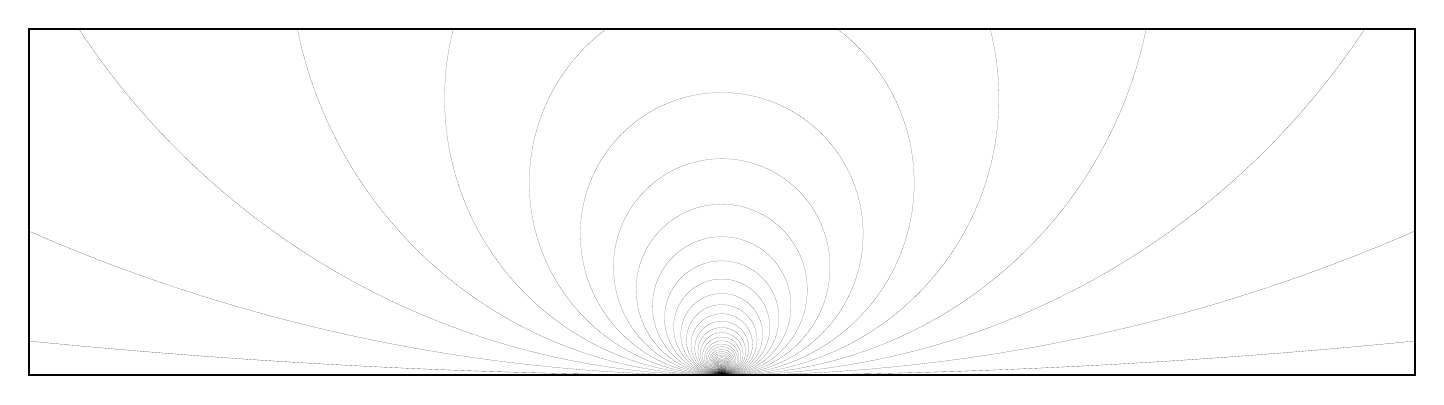
\begin{tikzpicture}[scale=88]
	\draw[thick] (-.1,0) rectangle (.1,.05);
	\clip (-.1,0) rectangle (.1,.05); % remove for all circles
	\foreach \i in {1,...,100}{
		\draw[line width=0.1/\i mm] (0, 1/\i^2) circle (1/\i^2);
	}
	\end{tikzpicture}
	\caption{A closeup of the Hawaiian hearing $\mathbb{H}^1$.}
	\label{fig:earrings}
\end{figure}

\begin{thm} \label{thm:counterexample}
	Let $\H$ be a homology theory such that its value on a point is finitely generated for every degree and on $\HE$ is not finitely generated for some degree. Then, the function $f \colon \HE \to \R$ whose value at the origin is $0$ and is $1$ everywhere else defines a $\HLC$ Morse filtration that is not q-tame.
\end{thm}

\begin{proof}
	The space $\HE$ is Hausdorff and locally compact since $R^{d+1}$ is.
	To verify that $(\HE,f)$ is a Morse filtration we notice that all level sets are either the empty set, the singleton containing the origin, or $\HE$ itself, all compact spaces.
	Let us now verify that $\HE$ is $\HLC$.
	Let $\epsilon > 0$ and $x \in \HE$.
	If $x$ is the origin, we choose $\delta$ between $0$ and the minimum of $\epsilon$ and $1$.
	Then $\HE_{\leq f(x) + \delta} = \HE_{\leq \delta} = \{x\}$, so the desired condition follows from the first assumption on the homology theory.
	For $x$ not the origin, there is a unique $d$-sphere that contains it.
	Clearly, we may choose $\delta > 0$ so small that $D_\delta(x) = \{y \in \R^{d+1} \mid \Vert x - y \Vert < \delta\} \cap \HE$ is contained in this sphere, so $D_\delta(x)$ is homotopy equivalent to a $x$ and the condition again follows trivially.
	What remains to be shown is that $\HE_{\leq \bullet}$ is not q-tame.
	Since $\HE_{\leq t}$ is constant with value $\HE$ for $t \geq 1$, the second assumption on the homology theory finishes the proof.
\end{proof}

The theories that we are most interested in do satisfy these conditions.

\begin{prop}
	The assumptions of Theorem~\ref{thm:counterexample} are satisfied by singular homology with any coefficients and \v{Cech} homology with field coefficients.
\end{prop}

\begin{proof}
	The case of singular homology is well know and can be found in \cite{Barratt.1962}.
	For \v{C}ech homology we use the fact that it commutes with inverse limits for compact Hausdorff spaces.
	Define 
	\begin{align*}
	\HE_k &= \left\{(x_0,\dots,x_d)\in\R^{d+1}\mid \left(x_0-\frac{1}{k}\right)^2+x_1^2+\dots+x_d^2=\left(\frac{1}{k}\right)^2\right\}\\
	&\cup\bigcup_{n=1}^{k-1}\left\{(x_0,\dots,x_d)\in\R^{d+1}\mid \left(x_0-\frac{1}{n}\right)^2+x_1^2+\dots+x_d^2=\left(\frac{1}{n}\right)^2\right\},
	\end{align*}
	i.e., the $d$-dimensional Hawaiian earring but with the $k$-th largest $d$-sphere filled.
	We have $\lim_{k}\HE_{k} = \bigcap_{k}\mathbb{H}^{d}_{k}=\mathbb{H}^{d}$, and hence $\CH_{d}(\HE) = \lim_{k}\CH_{d}(\mathbb{H}^{d}_{k})$.
	One can easily check that each $\mathbb{H}^{d}_{k}$ satisfies the assumptions for \cref{prop:cech_sing_hom_hlc}, which implies $\lim_{k}\CH_{d}(\mathbb{H}^{d}_{k})=\lim_{k}H_{d}(\mathbb{H}^{d}_{k})$.
	We compute
	\begin{equation*}
	\lim_{k}H_{d}(\mathbb{H}^{d}_{k})=\lim\left(\dots\to \prod_{n=1}^2\mathbb{F}\to \prod_{n=1}^1\mathbb{F}\to \prod_{n=1}^0\mathbb{F}\right)=\prod_{n\in\mathbb{N}}\mathbb{F},
	\end{equation*}
	which is infinite-dimensional over $\mathbb{F}$.
	This finishes the proof.
\end{proof}

Now we verify that Morse filtrations which are $\HLC$ are q-tame.
We will need three lemmas. 

\begin{lem} \label{l:commutative algebra}
	Given a commutative diagram of modules over a principal ideal domain
	\begin{equation*}
	\begin{tikzcd}
	A_{1,1} \arrow[r] & A_{1,2} & \\
	A_{2,1} \arrow[r] \arrow[u] & A_{2,2} \arrow[r] \arrow[u] & A_{2,3} \\
	& A_{3,2} \arrow[r] \arrow[u] & A_{3,3} \arrow[u]
	\end{tikzcd}
	\end{equation*}
	where the middle row is exact and both $A_{2,1} \to A_{1,1}$ and $A_{3,3} \to A_{2,3}$ have finitely generated images, then so does $A_{3,2} \to A_{1,2}$.
\end{lem}

\begin{proof}
	This is proven via a straightforward diagram chase. For more details see Lemma 17.3 in \cite{Bredon.1968}.
\end{proof}

\begin{lem} \label{l:neighborhood third}
	Let $X$ be locally compact space.
	For any compact subset $K$ and open set $U$ with $K \subseteq U$ there exists a compact set $K^\prime$ such that
	\begin{equation*}
	K \subseteq \interior(K^\prime) \subseteq K^\prime \subseteq U.
	\end{equation*}
\end{lem}

\begin{proof}
	For any $x \in K$ choose a compact neighborhood $C(x) \subseteq U$.
	We have
	\begin{equation*}
	K \subseteq \bigcup_K \interior(C(x)) \subseteq \interior\left(\bigcup_K C(x)\right) \subseteq \bigcup_K C(x) \subseteq U
	\end{equation*}
	Since $K$ is compact, the first inclusion above is achieved over a finite subset $\{x_1, \dots, x_m\}$ of elements in $K$.
	Defining $K^\prime = \bigcup_{i=1}^m C(x_i)$ finishes the proof.
\end{proof}

\begin{lem} \label{l:key lemma for q-tameness}
	Fix a homology theory. Let $(X,f)$ be a $\HLC$ Morse filtration.
	Consider sets $K, L \subseteq X$ with $K$ compact and $K \subseteq \interior(L)$. For any $s < t$ there is $\delta \in (0,\, t-s)$ such that $K \cap X_{s+\delta} \to L \cap X_{t}$ is $\HS$.
\end{lem}

\begin{proof}
	We need to prove that the inclusion $X_s \to X_t$ is $\HS$ for every $s < t$.
	
	The lemma holds for $\HS$ replaced by $\HS_{(n-1)}$ for any $n \leq 0$ since $\H_{n-1}$ induces the zero map. We will proceed by induction on $n$ assuming the lemma for $\HS_{(n-1)}$. 
	
	Given a compact set $L \subseteq X$ and $s < t$ let $\Sigma_{s, t}$ be the collection of all compact subsets $K$ of $\interior(L)$ for which there exists $\delta_K > 0$ and an open neighborhood $U(K)$ of $K$ such that $U(K) \cap X_{s+\delta_K} \to L \cap X_{t}$ is $\HS_n$.
	
	We start by showing that any element of $\interior(L) \cap X_s$ has a neighborhood in $\Sigma_{s, t}$.
	Let $x \in \interior(L) \cap X_{s}$.
	Consider an open neighborhood $U(x)$ of $x$ contained in $\interior(L)$, and take $\epsilon > 0$ such that $s + \epsilon < t$.
	By the strong $\HLC$ of $(X,f)$ there is a $\delta \in (0, \epsilon)$ and an open neighborhood $W(x) \subseteq U(x)$ such that for $c = s - f(x)$ the following composition is $\HS$:
	\begin{equation*}
	W(x) \cap X_{f(x) + c + \delta} \to
	U(x) \cap X_{f(x) + c + e} \to
	L \cap X_{t}.
	\end{equation*}
	By local connectivity we can choose a compact neighborhood of $x$ contained in $W(x)$.
	This proves the claim.
	
	We will now show that the class $\Sigma_{s,t}$ is closed under finite unions.
	For $i \in \{1, 2\}$ let $K_i$ be in $\Sigma_{s,t}$ with $\delta_i > 0$ and $K_i \subseteq U_i$ open such that $U_{i} \cap X_{s+\delta_i} \to L \cap X_{t}$ is $\HS_n$.
	We Use Lemma \ref{l:neighborhood third} to construct sets $K_i^\prime$ such that
	\begin{equation*}
	K_i \subseteq \interior(K_i^\prime) \subseteq K_i^\prime \subseteq U_i.
	\end{equation*}
	Notice that for $\delta = \min(\delta_i)$ we have $K_i^\prime \cap X_{s+\delta} \to L \cap X_t$ is $\HS_n$.
	Additionally, the induction hypothesis implies that $K_1 \cap K_2 \cap X_s \to K_1^\prime \cap K_2^\prime \cap X_{s+\delta}$ is $\HS_{(n-1)}$.
	We therefore have the following commutative diagram satisfying the assumptions of Lemma~\ref{l:commutative algebra}:
	\begin{equation*}
	\begin{tikzcd}
	\H_n(L \cap X_t) \oplus \H_n(L \cap X_t) \arrow[r] &
	\H_n(L \cap X_t) & \\
	\H_{n}(K_1^\prime \cap X_{s+\delta}) \oplus \H_n(K_2^\prime \cap X_{s+\delta}) \arrow[r] \arrow[u] & 
	\H_{n}((K_1^\prime \cap X_{s+\delta}) \cup (K_2^\prime \cap X_{s+\delta})) \arrow[r] \arrow[u] &
	\H_{n-1}(K_1^\prime \cap K_2^\prime \cap X_{s+\delta}) \\ & 
	\H_{n}((K_1 \cup K_2) \cap X_s) \arrow[r] \arrow[u] &
	\H_{n-1}(K_1 \cap K_2 \cap X_s). \arrow[u]
	\end{tikzcd}
	\end{equation*}
	We conclude that $K_1 \cup K_2 \in \Sigma_{s, t}$.
	Since any compact $K \subseteq \interior(L)$ can be expressed as a finite union of sets in $\Sigma_{s,t}$ the induction step and the lemma are proven.
\end{proof}

\begin{thm} \label{t:strong local connectenss implies q-tameness}
	Morse filtrations which are $\HLC$ give rise to q-tame persistence modules for any homology theory.
\end{thm}

\begin{proof}
	It follows from applying Lemma~\ref{l:key lemma for q-tameness} to $K = X_{\leq s}$ and $L = X$.
\end{proof}

%!TEX root = ../func_top.tex

\section{Persistent homology and functional topology} \label{s:surfaces}

Having established topological conditions for the existence of persistence diagrams associated to filtrations and corresponding generalized Morse inequalities, we now describe how these results relate to Morse's general theory of functional topology \cite{Morse.1937, Morse.1938, Morse.1940}, and to its application in Morse and Tompkins' work on unstable minimal surfaces from \cite{Morse.1939}.
We will focus on the homological aspects of this approach referring to \cite[Sections 4.3--5]{Bott.1980} for a general exposition.
For a more thorough presentation of the unstable minimal surface problem, including the analytical details, please consult \cite[Section II.6]{Struwe.1988}, and for a historical account and an overview of subsequent results see \cite[Section 6]{Dierkes.2010} and \cite[Section 6.8.1]{Dierkes.2010b}.

\subsection{The unstable minimal surface problem}

Morse and Tompkins considered the following setting introduced by Douglas.
Let $g \colon \R \to \R^n$ be a $2\pi$-periodic function representing a simple closed curve such that $g$ is differentiable with Lipschitz derivative.
Let $\widetilde{\Omega}$ be the space of continuous functions $\varphi \colon \R \to \R$ with $\varphi(t+2\pi) = \varphi(t) + 2\pi$ for all $t$ and $\varphi(\alpha_i)=\alpha_i$ for three fixed distinct points $\alpha_i \in [0,2\pi)$.
The \emph{Douglas functional} on $\widetilde \Omega$ associated to the curve $g$ is defined as
\begin{equation*}
A_g(\varphi) = \frac{1}{16 \pi} \int_0^{2\pi} \int_0^{2\pi}  \left\| \frac{g(\varphi(\alpha)) - g(\varphi(\beta))}{\sin \frac{\alpha-\beta}{2}} \right\|_2^2 \ \mathrm{d}\alpha \ \mathrm{d}\beta.
\end{equation*}
It coincides with the Dirichlet energy of the unique harmonic extension of the reparametrized curve $g \circ \varphi$ to a parametrized surface.
The Dirichlet energy is an upper bound for the area, with equality if the parametrization is conformal.
Let $\Omega_g = \{\varphi \in \widetilde\Omega \mid A_g(\varphi) < \infty\}$, equipped with the $C^0$ metric.
Douglas proved that, for a large class of curves~$g$, the set $\Omega_g$ is non-empty and the sublevel sets of $A_g$ are compact.
Since $A_g$ is bounded below by $0$, this implies that $A_g$ attains a global minimum.
The corresponding surface is then a solution of \emph{Plateau's Problem}, which asks for a surface homeomorphic to a disk with boundary $g$ and minimum area.

As alluded to in \cref{r:homotopically critial points}, Morse and Tompkins consider a homotopical notion of critical point for a general function $F \colon M \to \R$ on a metric space \cite[p.~445]{Morse.1939}, see also \cite{Morse.1943}.
Roughly, a point $p$ is \emph{homotopically critical} if it has no neighborhood in $M_{\leq F(p)}$ that can be mapped by a homotopy into $M_{\leq t}$ for some $t<F(p)$.

Morse and Tompkins prove \cite[p.~464]{Morse.1939} that each homotopically critical point of the functional $A_g$ indeed corresponds to
%
%a critical point of the area functional,
%called
a \emph{minimal surface} -- a surface with vanishing mean curvature -- and use this correspondence to prove the following result, also reviewed in \cite[Theorem II.6.10]{Struwe.1988}.

\begin{thm}[{Unstable Minimal Surface Theorem \cite[p.~472]{Morse.1939}}]
	If the space $\Omega_g$ contains two distinct solutions of Plateau's Problem contained in disjoint critical sets of the functional $A_g$, then it also contains a critical set not of minimum type.
	%, more precisely, a homotopically critical point of $A_g$ of non-minimum type.
\end{thm}
Here, a \emph{critical set} $S$ is a closed and open subspace of the set of all critical points with a given function value.
It is said to be of \emph{minimum type} if for every neighborhood $N$ of $S$, the function value on the complement $N \setminus S$ exceeds the function value on $S$.
%it corresponds to a homotopically critical point of $A_g$ of non-minimum type?
In addition to the general theorem above, Morse and Tompkins also give an explicit example of a curve $g$ satisfying the assumptions, thus proving the existence of an unstable minimal surface in the above sense.

%sci-hub.se/10.1215/S0012-7094-41-00828-1
%
%A point q of M will be termed non-minimizing if in every neighborhood of q there is a point p such thatF(p)<F(q). A homotopic critical set which is not a minimizing set contains at least one non-minimizing point of F.

While more efficient and more general proofs for the existence of an unstable minimal surface (with respect to more natural topologies than $C^0$) have subsequently been established \cite{Struwe.1988,Dierkes.2010}, including less restrictive assumptions on the boundary curve, the original approach of Morse and Tompkins is notable for its close connection to persistent homology.


\subsection{Morse's local connectivity conditions}

Parts of the framework of functional topology that Morse and Tompkins use is developed by Morse in \cite{Morse.1940} in a very general setting.
In particular, he proves inequalities for cap numbers associated to the persistent \v{C}ech homology of the sublevel set filtration, as also considered in \cref{s:inequalities}.
From these generalized Morse inequalities, the existence of an unstable minimal surface can easily be deduced in the presence of two distinct critical sets of minimum type.

We have seen that these inequalities require q-tameness, so in order to apply them in the minimal surface setting % and deduce their theorem,
one needs to prove the \mbox{q-tameness} of the sublevel set filtration of the Douglas functional $A_g$.
Throughout his work on functional topology, in order to obtain \mbox{q-tameness}, Morse assumed slightly varying forms of local connectivity on the resulting sublevel set filtrations.
In particular, Morse and Tompkins used the following condition in their applications to minimal surface theory (see also \cite[p.~ 25]{Morse.1938} and \cite[p.~464]{Morse.1939}, but note that the definitions given there contain typographical errors):
\begin{displaycquote}[p.~431]{Morse.1940}
%\cite[p.~ 25]{Morse.1938}
	Let $p$ be a point of $M$ at which $F(p)=c$.
	The space $M$ is said to be \emph{locally $F$-connected} of order $r$ at~$p$ if corresponding to each positive constant $e$ there exists a positive constant $\delta$ such that each singular $r$-sphere on the $\delta$-neighborhood of $p$ and on $F_{c+\delta}$ bounds an $(r+1)$-cell of norm $e$ on $F_{c+e}$.
\end{displaycquote}
Using similar language to the one used in \cref{s:connectivity}, the property of local $F$-connectedness of all orders is equivalent to the following notion applicable to general topological spaces.

\begin{defi}
	The sublevel set filtration of a function $f \colon X \to \R$ is said to be \emph{weakly homotopically locally connected}, or \emph{weakly $\piLC$}, if for any $x \in X$, $V$ a neighborhood of $x$, and any index $t > f(x)$, there is an index $s$ with $f(x) < s < t$ and a neighborhood $U$ of $x$ with $U \subseteq V$ such that the inclusion $f_{\leq s} \cap U \to f_{\leq t} \cap V$ induces trivial maps on homotopy groups.
\end{defi}

Morse then goes on to claim that the persistent \v{C}ech homology of this sublevel set filtration is q-tame, provided that $F$ is bounded from below and satisfies the assumptions of local $F$-connectivity and compactness of sublevel sets.
%, and a further condition called $F$-regularity, which is trivially satisfied if the domain of $F$ is compact.
In the original (where the function is assumed to take values in $[0,1)$) the claim reads:
\begin{displaycquote}[Theorem 6.3, p.~432]{Morse.1940}
	Let $a$ and $c$ be positive constants such that $a < c < 1$.
	The $k^{\mathrm{th}}$ connectivity $R^k(a,c)$ of $F_a$ on $F_c$ is finite.
\end{displaycquote}
Morse does not prove this statement in the given reference, but rather refers to \cite[Theorem~6.1]{Morse.1938}.
Unfortunately, the above claim does not hold in general, as exemplified by the sublevel set filtration from \cref{t:counterexample}.
To elaborate on this, we consider a stronger version of weak local connectedness.

\begin{defi}
	The sublevel set filtration of a function $f \colon X \to \R$ is said to be \emph{weakly locally connected} or weakly $\LC$ if for any $x \in X$, $V$ a neighborhood of $x$, and any index $t > f(x)$, there is an index $s$ with $f(x) < s < t$ and a neighborhood $U$ of $x$ with $U \subseteq V$ such that the inclusion $f_{\leq s} \cap U \to f_{\leq t} \cap V$ is homotopic to a constant map.
\end{defi}

Clearly, being weakly $\LC$ implies being weakly $\piLC$ and, if the homology $\H$ takes finite dimensional values on one-point spaces, also weakly $\HLC$.
Observe that the proof of \cref{t:counterexample} actually establishes that the filtration given there is weakly $\LC$, so not even the weak $\LC$ condition is sufficient to ensure the q-tameness of compact sublevel set filtrations that are induced by non-continuous functions in general.
In particular, our construction invalidates Morse's claim quoted above because \v{C}ech homology satisfies the assumptions on the homology theory made in \cref{t:counterexample}.

Specifically, using the the fact that \v{C}ech homology of compact Hausdorff spaces commutes with inverse limits, it is straightforward to verify that the \v{C}ech homology in degree $d$ of the $d$-dimensional Hawaiian earring is isomorphic to $\prod_{n\in\N}\F$, which is infinite dimensional over $\F$.
%To see that his is the case, one can use the fact that \v{C}ech homology commutes with totally ordered limits for compact Hausdorff spaces \cite[Theorems VIII.3.6 and X.3.1]{Eilenberg.1952} as follows.
%Define
%\begin{align*}
%\HE_k &=
%\left\{ (x_0, \dots, x_d) \in \R^{d+1} \ \middle| \ \left( x_0 - \frac{1}{k} \right)^2 + x_1^2 + \dots + x_d^2 \leq \left( \frac{1}{k} \right)^2 \right\} \\ &\, \cup
%\bigcup_{n=1}^{k-1} \left\{ (x_0, \dots, x_d) \in \R^{d+1} \ \middle |\ \left( x_0 - \frac{1}{n} \right)^2 + x_1^2 + \dots + x_d^2 = \left( \frac{1}{n} \right)^2 \right\},
%\end{align*}
%i.e., the $d$-dimensional Hawaiian earring but with the $k$-th largest $d$-sphere filled.
%We have $\lim_{k} \HE_{k} = \bigcap_{k} \HE_{k} = \HE$, and hence $\CH_{d}(\HE; \F) = \lim_{k} \CH_{d}(\HE_{k}; \F)$, where $\CH$ denotes \v{C}ech homology.
%Clearly, each $\HE_{k}$ is a CW-complex, so we can simply use cellular homology to compute
%\begin{equation*}
%\lim_{k}\CH_{d}(\mathbb{H}^{d}_{k}; \F)=\lim\left(\dots\to \prod_{n=1}^2\F\to \prod_{n=1}^1\F\to \prod_{n=1}^0\F\right)=\prod_{n\in\N}\F,
%\end{equation*}
%which is infinite-dimensional over $\F$.
%We will consider the \emph{$d$-dimensional Hawaiian earring}
%\begin{equation*}
%\HE = \bigcup_{n \in \N} \left\{ (x_0, \dots, x_d) \in \R^{d+1} \ \middle | \ \left( x_0 - \frac{1}{n} \right)^2 \!\! + x_1^2 + \dots + x_d^2 = \left( \frac{1}{n} \right)^2 \right\},
%\end{equation*}
%which is a compact subspace of $\R^{d+1}$.
%
%\begin{figure}[t]
%	\centering
%	\begin{tikzpicture}[scale = 60]
%	\draw[thick] (-.1,-.001) rectangle (.1,.05);
%	\clip (-.1,0) rectangle (.1,.05);
%	\foreach \i in {1,...,100}{
%		\draw[line width=0.4/\i^0.25 pt] (0, 1/\i^2) circle (1/\i^2);
%	}
%	\end{tikzpicture}
%	\caption{A closeup of the Hawaiian earring $\mathbb{H}^1$.}
%\end{figure}
%
%\begin{thm} \label{t:counterexample}
%	The function $f \colon \HE \to \R$ whose value at the origin is $0$ and is $1$ everywhere else defines a compact and weakly $\LC$ sublevel set filtration that is not q-tame with respect to $\H$ if $\H_{n}(\HE)$ is infinite dimensional for some $n$.
%\end{thm}
%
%\begin{proof}
%	To verify that $f$ has compact sublevel sets we notice that all sublevel sets are either the empty set, the singleton containing the origin, or $\HE$ itself, all compact Hausdorff spaces.
%
%	In order to verify that the sublevel set filtration of $f$ is weakly $\LC$, we
%	consider $x \in \HE$, $V$ a neighborhood of $x$ in $\HE$ and $t > f(x)$. We need to find a neighborhood $U \subseteq V$ of $x$ and $s \in (f(x), t)$ such that the inclusion $f_{\leq s} \cap U \to f_{\leq t} \cap V$ is homotopic to a constant map.
%
%	If $x$ is the origin, we have $f(x) = 0$ and choose $s \in (0, \min\{t, 1\})$.
%	Then $f_{\leq s} = \{x\}$, so with $U = V$ the inclusion $f_{\leq s} \cap U \to f_{\leq t} \cap V$ is the inclusion of $\{x\}$ into $f_{\leq t} \cap V$, which is a constant map, so the weak $\LC$ condition is trivially satisfied.
%
%	For $x$ not the origin we have $f(x) = 1$ and choose $s \in (1,t)$ arbitrarily, so that $f_{\leq s} = f_{\leq t} = \HE$.
%	Note that since $x$ is not the origin, there is a unique $d$-sphere in $\HE$ that contains $x$.
%	Clearly, we may choose $\delta > 0$ so small that $B_{\delta}(x) = \{y \in \R^{d+1} \mid \Vert x - y \Vert < \delta\} \cap \HE$ is a topological ball contained in this sphere and contained in $V$.
%	The ball $B_\delta(x)$ can be contracted to $\{x\}$ in $V$, so choosing $U = B_{\delta}(x)$, we obtain that the inclusion $f_{\leq s} \cap U \to f_{\leq t} \cap V$ is homotopic to the constant map with value $x$.
%
%	It remains to be shown that $f_{\leq \bullet}$ is not q-tame for $\H$.
%	This follows directly from our assumption that $\H_{n}(\HE)$ is not finite dimensional for some $n$, as $f_{\leq t}$ is constant with value $\HE$ for $t \geq 1$.
%\end{proof}
Moreover, the singular homology of the $d$-dimensional Hawaiian earring is also infinite dimensional, as proven in \cite{Barratt.1962}. In summary, we have the following.

\begin{cor} \label{c:counterexample}
	The function $f \colon \HE \to \R$ with value~$0$ at the origin and $1$ elsewhere defines a weakly $\LC$ compact sublevel set filtration that is not q-tame with respect to singular and \v{C}ech homology.
\end{cor}

The gap we have thus highlighted in the argument of Morse and Tompkins, that the sublevel set filtration of $A_g$ is not necessarily q-tame, can be fixed by applying \cref{t:local connectedness implies q-tameness}.
This is because the proof given in \cite[p.464]{Morse.1939} for the local connectivity of the sublevel set filtration induced by $A_g$ can actually be seen to establish a stronger property described next.

\begin{defi}
	The sublevel set filtration of a function $f \colon X \to \R$ is said to be $\LC$ if for any $x \in X$, any neighborhood $V$ of $x$ and any pair of indices $f(x) < s < t$ there is a neighborhood $U \subseteq V$ of $x$ such that the map $f_{\leq s} \cap U \to f_{\leq t} \cap V$ is homotopic to a constant map.
\end{defi}

Clearly, the filtration being $\LC$ implies that the filtration is also $\HLC$ for \v{C}ech homology with field coefficients, which is the homology theory Morse and Tompkins use.
Therefore, from \cref{t:local connectedness implies q-tameness} we can conclude that the sublevel set filtration of $A_g$ is indeed \mbox{q-tame} as needed.
This implies that the generalized Morse inequalities hold, and hence so does the Unstable Minimal Surfaces Theorem.

We have also mentioned that Morse introduced another condition that he also called local $F$-connectivity three years earlier.
It roughly corresponds to being $\piLC$ with a certain added uniformity property.
In the original it reads:
\begin{displaycquote}[p.421--422]{Morse.1937}
	The space $M$ will be said to be locally $F$-connected for the order $n$ if corresponding to $n$, an arbitrary point $p$ on $M$, and an arbitrary positive constant $e$, there exists a positive constant $\delta$ with the following property.
	For $c \geq F(p)$ any singular $n$-sphere on $F \leq c$ (the continuous image on $F \leq c$ of an ordinary $n$-sphere) on the $\delta$-neighborhood $p_{\delta}$ of $p$ is the boundary of a singular $(n + 1)$-cell on $F \leq c + e$ and on $p_e$.
\end{displaycquote}
Morse also claims in the given reference that this condition is sufficient for q-tameness, but without providing a proof.
Whether this statement is true or not is not covered by our analysis, because the $\piLC$ and $\HLC$ conditions generally do not imply each other.
We expect the quoted claim to be true, but do not investigate it further.

\appendix

\section{Vietoris and \v{C}ech homology} \label{s:vietoris}

An interesting aspect of Morse's work from the modern point of view is his use of metric Vietoris homology with coefficients in a field, which closely relates to the use of filtered Vietoris-Rips and \v{C}ech complexes in topological data analysis.

For greater generality, instead of metric Vietoris homology we have instead considered \v{C}ech homology in the previous section.
We now justify this choice showing that these two homology constructions agree on compact metric spaces.

First, let us recall the definition of \v{C}ech homology as presented for example by \citet[Section IX--X]{Eilenberg.1952}.
Let $X$ be a topological space and let $\Cov(X)$ be the set of all open covers of $X$ ordered by the refinement relation. 
Recall that for an open cover $\alpha \in \Cov(X)$ its \emph{nerve} $\Nrv(\alpha)$ is defined as the simplicial complex
\begin{equation*}
\Nrv(\alpha) =
\big\{ \beta \subseteq \alpha \mid \beta \text{ is finite and } \textstyle{\bigcap_{U \in \beta}} \, U \neq \emptyset \big\}.
\end{equation*}
The nerve construction defines a functor from the poset $\Cov(X)$ regarded as a category to that of simplicial complexes. 
The \emph{\v{C}ech homology with coefficients in $\mathbb{F}$} of $X$ is defined as
\begin{equation*}
\CH(X; \mathbb{F}) \ =
\lim_{\alpha \in \Cov(X)} H(\Nrv(\alpha); \mathbb{F}).
\end{equation*}
As an alternative to the nerve construction, for a cover $\alpha \in \Cov(X)$ one can define $\Vietoris(\alpha)$ as the simplicial complex
\begin{equation*}
\Vietoris (\alpha) = \left\{ \sigma \subseteq X \mid \sigma \text{ is finite and } \sigma \in U \text{ for some } U \in \alpha \right\},
\end{equation*}
which again yields a functor from $\Cov(X)$ to simplicial complexes.
This construction is dual in the sense of Dowker's Theorem \cite{Dowker.1952} to the nerve construction.
As a consequence, we have that $H (\Nrv (\alpha); \mathbb{F}) \cong H (\Vietoris (\alpha); \mathbb{F})$.
This isomorphism is natural with respect to refinement so we get an alternative description of \v{C}ech homology as 
\begin{equation*}
\CH (X; \mathbb{F}) \ \cong
\lim_{\alpha \in \Cov (X)} H (\Vietoris (\alpha); \mathbb{F}).
\end{equation*}

If $X$ is a metric space, this is still not exactly the same as the construction of metric Vietoris homology presented in \cite{Vietoris.1927} and used by Morse, which in modern notation is the limit
\begin{equation*}
\lim_{\alpha \in \Balls(X)} H (\Vietoris (\alpha); \mathbb{F}),
\end{equation*}
where 
\begin{equation*}
\Balls (X) = \left\{ ( B_{\delta} (x) )_{x \in X} \mid \delta > 0 \right\}
\subseteq \Cov (X).
\end{equation*}
However, if the metric space $X$ is compact, then $\Balls (X)$ is coinitial in $\Cov (X)$, that is to say, they both define the same limit.
Thus, we have a natural isomorphism
\begin{equation*}
\CH (X; \mathbb{F}) \ \cong \,
\lim_{\alpha \in \Balls(X)} H (\Vietoris (\alpha); \mathbb{F})
\end{equation*}
for a compact metric space $X$.
In other words, the metric Vietoris homology theory employed in Morse's setting is canonically isomorphic to the \v{C}ech homology we considered.


\section*{Acknowledgements}
This research has been supported by German Research Foundation (DFG) through the Collaborative Research Center SFB/TRR 109 \emph{Discretization in Geometry and Dynamics}, the Collaborative Research Center SFB/TRR 191 \emph{Symplectic Structures in Geometry, Algebra and Dynamics}, the Cluster of Excellence EXC-2181/1 \emph{STRUCTURES}, and the Research Training Group RTG 2229 \emph{Asymptotic Invariants and Limits of Groups and Spaces}.

A.M-M. acknowledges financial support from Innosuisse grant \mbox{32875.1 IP-ICT-1} and the hospitality of the Laboratory for Topology and Neuroscience at EPFL, where part of this work developed.

\bibliographystyle{abbrvnaturl}
\bibliography{biblio}

\end{document}